\section{Admission-benchmarks/Grade \% Correlation}
Correlation coefficients ($r$) between different admissions benchmarking methods and CSC1015F course results are worked out for students that are South African citizens or permanent residents, and that attended CSC1015F during their undergraduate career. Correlation is worked out on retrieval of the dataset comprising a join of admissions and grade data. In terms of SQL, such a join can be described as a \textit{left outer join} in which rows of the benchmark data are joined to rows of the grade data on the student number field; a single student may have many grade results (for example, when repeating a course) but only has a single row in the admissions data for the year in which the student first registered.

\subsection{ETL}
Using nETL, rows are extracted from the two CSV files (\textit{Admissions (2014 - 2016).csv} and \textit{Grades (2014 - 2016).csv}) independently of each other and concurrently, in batches of 5 000 and 10 000 rows respectively.

Via nETL configuration, rows from the admissions data are selected for students that are South African citizens or permanents residents, and that are undergraduates. Rows from the grades data are selected for students that attended CSC1015F during their undergraduate career. Because this information is not available in the admissions data, dynamic filter is applied to the admissions data to further select students that meet this same criteria. The CSV data represented as objects contains numerous fields that are not required, and so nETL is configured to apply an attribute-whitelisting process to both admissions and grade data. Batches of objects are serialized to JSON strings and loaded into a single CouchDB database via the \textit{\_bulk\_docs} endpoint. An example of a row from grade data serialized to a JSON string and as loaded into CouchDB is shown in Figure \ref{fig-json-grade}

\begin{figure}[H]
  \centering
  \begin{mdframed}
    \centering
    \begin{minted}{text}
{
  "_id": "7530f4eed7e6bc3ef0d99a53be8ba9a2",
  "_rev": "8-232d0cf39728d41b4c5935f12469209d",
  "RegAcadYear": 2016,
  "RegTerm": 1161,
  "anonIDnew": 1,
  "RegCareer": "UGRD",
  "Degree": "QHB002",
  "Course": "PHI1010S",
  "CourseSuffix": "S",
  "Percent": "55",
  "CourseID": 109157,
  "Dept": "PHI",
  "type_": "grade"
}    
        \end{minted}
  \end{mdframed}
  \caption[Grade Document JSON Sample]{\textbf{Figure \ref{fig-json-grade}: Example of a single line from the \textit{Grades (2014 - 2016).CSV} file}}
  \label{fig-json-grade}
\end{figure}

\subsection{Index Calculation}
Following loading the data from the CSVs into CouchDB, a Map function is used to produce an index of the CouchDB documents ordered by Student ID, with the guarantee that for every unique student id documents are ordered by type; the demographic document precedes the Grade documents for any given student. Knowing the order of documents via the view-index allows for performing the join on data-retrieval. Only a map function is used is required (no reduce function). That is, on Map function execution the ``type\_'' attribute is checked. If the document is a line of the Grades entity, then the key [Student ID, Course, year] is emitted along with a single number for the value - the percent achieved for the course. If the document is a line of the Benchmarks entity, then the key [student ID, 0, 0] is emitted along with an ordered list of 8 values corresponding to each of the 19 different methods of benchmarking students.

Normalization of the percentage fields (i.e. ``Percent'' for the Grades entity and the test results in the Benchmarks entity) is done via a nested function (a function defined within the map function) according to best-guess logic on how grade symbols correlate with percentage - the logic used for this is shown in Table \ref{ap-tbl-normalize-grades} and Table \ref{ap-tbl-normalize-admissions} in the appendix.

Because a student should only be represented by a single row in the admissions data and should only achieve a single grade per course per year, this 2-way join is achievable without using a reduce function. There is also no need to aggregate rows from either the admissions or grade data prior to joining. Logic of the map function is shown in the activity diagram in Figure \ref{fig-mapfn-correlation-grades}.

\begin{figure}[H]
    \centering
    \begin{mdframed}
        \centering
        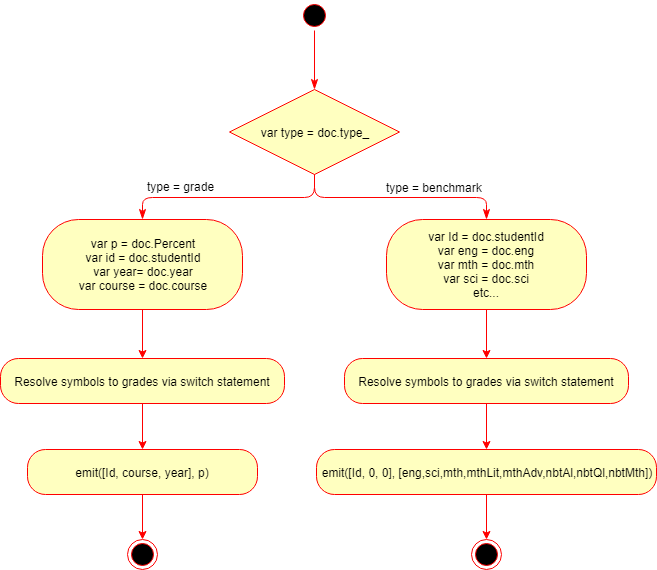
\includegraphics[scale=0.59]{./resources/figures/fig-mapfn-correlation-grades.png}
    \end{mdframed}
    \caption[\textit{Map}-function: \texorpdfstring{grades $\bowtie$ admissions}{Lg}]{\textbf{Figure \ref{fig-mapfn-correlation-grades}: \textit{Map}-function: \texorpdfstring{grades $\bowtie$ admissions}{Lg}}}
    \label{fig-mapfn-correlation-grades}
\end{figure}


\subsection{Index Retrieval}
The join of admissions and grade data is performed during index retrieval via a CouchDB list function.

On invocation the CoucDB list function opens and scans the index iteratively processing each document (i.e. iteratively processing each student; first a student's demographic document is processed, then a student's grades documents are processed). The 2-way join is achieved in this way; for every student number the grade and admissions data is joined, and summations of various fields of the grades and each benchmark are updated. Once the iteration over student numbers is finished, the summations are used to calculate correlation coefficients for each grade/benchmarking method combination according to the formula\footnote{\textit{x}: grade \%, \textit{y}: benchmark (\textit{r} is calculated for multiple \textit{y} values)}: \begin{spreadlines}{15pt}
    \begin{gather*}
        \intertext{\textit{Pearson Correlation Coefficient:}}
        r = \frac{N\sum{xy} - (\sum{x})(\sum{y})}{\sqrt{[N\sum{x^2} - (\sum{x})^2][N\sum{y^2} - (\sum{y})^2]}}
    \end{gather*}
\end{spreadlines}

Although the \_stats reduce function calculates \textit{sum of squares} per dataset, this is not useful in the case where individual rows from separate entities should be joined (such as in this 2-way join). For example, in reference to working out the numerator as provided in the correlation formula: \begin{spreadlines}{15pt}
    \begin{gather*}
        N\sum{xy} - (\sum{x})(\sum{y})
    \end{gather*}
\end{spreadlines}

Using CouchDB's \_stats function only the $\sum{x}$ and $\sum{y}$ values are accessible when joining the two entities during list function execution, and not $x$ and $y$ values (similarly, the denominator of the formula could also not be calculated from \_stats function output).

The list function is configured to output a table of correlation coefficients for each benchmarking method as shown in Table \ref{tbl-correlation-grades} (but in HTML format). List function logic is represented by the activity diagram in Figure \ref{fig-listfn-correlation-grades}.

\begin{figure}[H]
    \centering
    \begin{mdframed}
        \centering
        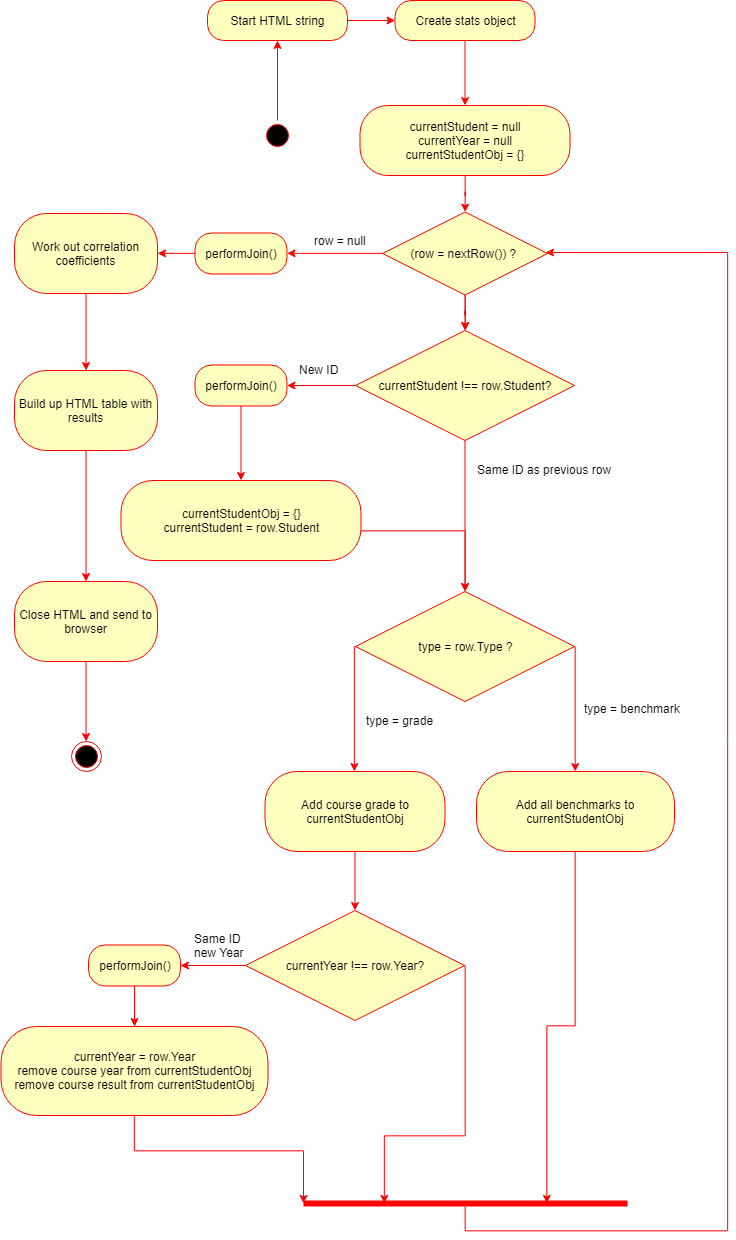
\includegraphics[scale=0.5]{./resources/figures/fig-listfn-correlation-grades.png}
    \end{mdframed}
    \caption[Grade/Benchmark correlation list function]{\textbf{Figure \ref{fig-listfn-correlation-grades}: Join/stats logic for grade/benchmark correlation analysis}}
    \label{fig-listfn-correlation-grades}
\end{figure}

\begin{table}[H]
    \begin{threeparttable}
        \textbf{Table \ref{tbl-correlation-grades}}\par\medskip\par\medskip
        \caption{Correlation between different benchmarking methods and CSC1015F grades}
        \label{tbl-correlation-grades}
        \begin{tabularx}{\textwidth}{>{\hsize=1.3\hsize}X>{\hsize=0.7\hsize}Y}
            \toprule
            \mC{c}{Benchmark}                     & \mC{c}{$r$} \\
            \midrule
            Gr12 Eng \%                           & 0.287       \\
            Gr12 Sci \%                           & 0.465       \\
            Gr12 Mth \%                           & 0.447       \\
            NBT AL \%                             & 0.368       \\
            NBT QL \%                             & 0.533       \\
            NBT Mth \%                            & 0.510       \\
            Avg Gr12 \%                           & 0.485       \\
            Avg Gr12 \% (Dbl Mth)                 & 0.487       \\
            Avg Gr12 \% (Dbl Mth \& Sci)          & 0.493       \\
            Avg NBT \%                            & 0.583       \\
            Avg NBT \% (Dbl AL)                   & 0.559       \\
            Avg NBT \% (Dbl QL)                   & 0.580       \\
            Avg NBT \% (Dbl Mth)                  & 0.583       \\
            Avg NBT \% (Dbl AL/QL)                & 0.567       \\
            Avg NBT \% (Dbl AL/Mth)               & 0.570       \\
            Avg NBT \% (Dbl QL/Mth)               & 0.589       \\
            Avg Gr12 \& NBT                       & 0.610       \\
            Avg Gr12 \& NBT (Dbl Gr12 Mth)        & 0.587       \\
            Avg Gr12 \& NBT (Dbl Gr12 Mth \& Sci) & 0.578       \\
            \bottomrule
        \end{tabularx}
    \end{threeparttable}
\end{table}



